\section{多源气象特征与区域异常因素识别}
\label{q1-sec}

\subsection{比较对象与多尺度特征}

本问识别事件参考时段相对于同季节背景的气象异常，得到供结构水热分析使用的候选因素。综合三种统计路线，主质量轨的前五项依次为土壤水分、空气湿状态、土壤热状态、空气热状态和平均风；其中第五席与土热通量存在竞争。排序表示区域观测的相对异常及其稳定性，物理作用还需结合源区条件解释。

使用吉隆地气相互作用逐小时综合观测的气象、辐射、土壤及通量四类资料\cite{q1-data}。元数据站址为$28.86^\circ$N、$85.29^\circ$E，海拔$4140\,\mathrm m$，对应区域背景站。主质量轨仅接纳有限且原始QC为0的值；无配对QC的降水和FLUX变量另列探索轨，原有非零QC值仍剔除。由63个原始变量构造24个驱动量、112个排序特征，其中82个属于主质量轨，另30个用于探索（表\ref{q1-tab-features}）。按物理对象归族，可防止同一变量的多个高度或统计量获得额外选票。

\begin{table}[htbp]
\centering\small
\caption{四类资料与特征库规模}
\label{q1-tab-features}
\begin{tabular}{lrrrrl}
\toprule
资料 & 原变量 & 驱动量 & 主轨特征 & 探索增量 & 主要表征\\
\midrule
MET  &22&10&37&5&温湿、平均风、气压、降水标签\\
RADM &4&4&20&0&长短波及上下行差\\
SOIL &12&5&25&0&浅层水热、垂向梯度、土热通量\\
FLUX &25&5&0&25&VPD、感潜热、摩擦速度、湍动能\\
\midrule
合计 &63&24&82&30&9个主轨族、3个新增探索族\\
\bottomrule
\end{tabular}
\parbox{\linewidth}{\footnotesize 注：探索轨保留主轨并加入30个特征；VPD并入空气湿状态。降水标签的积分时段、通量符号及处理口径按原资料保留，因此不计算累计降水或积分能量。}
\end{table}

参考时刻取题面所述时刻，按源时钟UTC+8换算为2026年8月26日02:30 UTC。取其前24、72和168小时的标签窗口；小时标签的平均区间边界仍作为时间口径条件。2021--2025年各取8月26日前后30天、每日一个同钟点背景，共305个窗口，按7日块划分45个天气过程代理。三日和十四日块用于敏感性分析，过程块只表征相关性，不计作灾害事件。

普通驱动量提取中位数、5\%和95\%分位数、每24小时线性趋势、最长连续上升链占窗口标签数的比例；风向以正余弦中位数表示。降水另取中位数、95\%分位数、最大值、有效值中的正值比例和最长正值链比例。缺测打断连续链，主设置要求窗口有效支持率至少75\%。这种设计同时保留状态、尾部与变化过程，避免只用单一极值代表整个事前窗口。

\subsection{三条异常路线与共识排序}

三条路线分别衡量边际偏离、条件异常和类比背景差异。对年份$y$中的过程$p$及其第$i$个有效窗口，令权重$w_i=1/(Y P_y n_{yp})$，其中$Y$为有效年份数，$P_y$为该年有效过程数，$n_{yp}$为过程内有效窗口数；遇缺测重新归一。路线A使用加权中点经验分布：
\begin{equation}
 F_j(x)=\sum_i w_i\!\left[\mathbf1(x_{ij}<x)+\tfrac12\mathbf1(x_{ij}=x)\right],
 \qquad a_j=2\left|F_j(x_j^*)-\tfrac12\right|.
 \label{q1-eq-ecdf}
\end{equation}
先在驱动量内取特征分数中位数，再在族内取驱动量分数中位数。中点处理允许常值背景，双侧距离则同时识别偏高和偏低异常。

路线B选取背景加权观测率至少80\%、覆盖至少三个年份且目标有值的列。以训练加权中位数为中心、$1.4826\,\mathrm{MAD}$为尺度，退化时改用$\mathrm{IQR}/1.349$，仍为零则剔除。训练中位数填补缺测，截断至$[-8,8]$并减去训练加权均值。借鉴协方差收缩思想\cite{q1-shrinkage}，固定单位阵目标及收缩强度：
\begin{equation}
 \Sigma_\lambda=(1-\lambda)C+\lambda I,\quad P=\Sigma_\lambda^{-1},\quad
 b_g=\frac{\eta_g^{\mathsf T}(P_{gg})^{-1}\eta_g}{d_g},\quad
 \eta=P\delta,\qquad\lambda=0.5.
 \label{q1-eq-conditional}
\end{equation}
这里$C$为加权协方差，$\delta$为中心化后的目标向量，$d_g$为族$g$的有效特征数。$b_g$表示给定其他族后的单位维数条件距离，再用逐年留出的背景贡献分布转换成上侧百分位；各族贡献不要求可加。每折重新确定选列、中心、尺度、填补和协方差，留出行须实际观测到该族全部活跃列才参与校准。

路线C以自然类比思想\cite{q1-analog}比较相近的其他气象状态：匹配空间沿用B的有效列，距离排除待评估族及其派生量，各剩余族等权；匹配维度实际观测率至少80\%，每年选取两个不同过程的最近窗口，至多10个类比。随后计算待评估族在类比集合中的双侧中点分布偏离，仍取驱动量、物理族两层中位数。该路线比较其他状态相近时，待评族的异常是否仍然突出。

三路线各自在每个窗口内形成名次$r_{gmw}$，同分用中间名次；跨路线、跨窗口的共识为
\begin{equation}
 S_g=\frac{1}{9}\sum_{w\in\{24,72,168\}}\sum_{m\in\{A,B,C\}}
 \left(1-\frac{r_{gmw}-1}{G_{mw}-1}\right).
 \label{q1-eq-consensus}
\end{equation}
主轨$G_{mw}=9$。TOP5边界出现并列时按剩余席位分配入选份额，避免用变量顺序打破并列。先做留年与留过程检查，后者按最大168小时实际标签支持清除相邻重叠窗口；两质量轨、三窗口共300个评估折，复用同样的50种分组。目标时段只用于评分，不参与尺度或参数选择。

五个留年折各以244个窗口训练、61个窗口留出；45个留过程折各以286--294个窗口训练、5--7个留出，并清除6--12个相邻窗口。分割单位保持年份与天气过程的组织结构，可减少重叠长窗口造成的近邻重复。它们服务于背景评分与排序检查，统计对象始终是同一案例的气象背景比较。

\subsection{排序结果与水热状态解释}

表\ref{q1-tab-ranks}给出三路线跨窗口排序和最终共识。A首先识别土水、空气热与短波，B更突出土热和空气湿，C更突出土水与平均风。路线差异说明边际偏离与其他气象状态给定后的异常并不等价；采用等权名次共识，可使不同量纲的路线分数具有一致的汇总尺度。

\begin{table}[htbp]
\centering\small
\caption{主质量轨的三路线跨窗口名次、共识及稳定性}
\label{q1-tab-ranks}
\begin{tabular}{lrrrrr}
\toprule
物理族 & A名次 & B名次 & C名次 & 共识$S_g$ & 平均入选频率\\
\midrule
\textbf{土壤水分}   &1&5&1&0.743&0.814\\
\textbf{空气湿状态} &5&2&3&0.667&0.814\\
\textbf{土壤热状态} &6&1&4&0.639&0.843\\
\textbf{空气热状态} &2.5&3&5&0.611&0.890\\
\textbf{平均风}     &8&4&2&0.583&0.527\\
\midrule
土热通量 &4&6&6&0.465&0.559\\
短波辐射 &2.5&8.5&7&0.410&0.304\\
长波辐射 &7&7&8&0.264&0.232\\
气压     &9&8.5&9&0.118&0.015\\
\bottomrule
\end{tabular}
\parbox{\linewidth}{\footnotesize 注：各路线名次由三窗归一名次得分平均后再排序，$S_g$由式\eqref{q1-eq-consensus}给出。频率为三窗内有效共识重采样的TOP5份额均值，每窗分母44、请求数100；它描述排序稳定性。}
\end{table}

图\ref{q1-fig-state}将实际轨迹与相对背景位置并列，体积含水率均以$\mathrm{m^3\,m^{-3}}$计。0.1米深度的168小时中位数为0.12103，处于季节背景约0.822的位置；同时首末值由0.1647降至0.08275，线性拟合显示每24小时下降约0.01222。因此，“背景位置较高”与“近期下降”同时成立，土水排名靠前应结合含水状态、梯度和趋势理解，不据此推导近期持续增湿。

\begin{figure}[htbp]
\centering
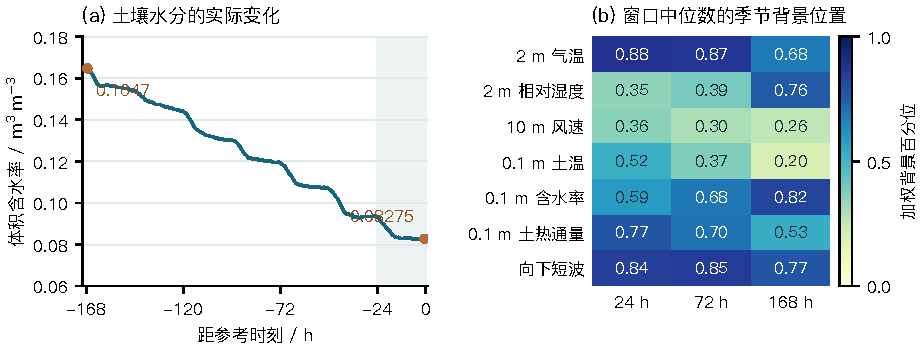
\includegraphics[width=\linewidth]{figures/q1/q1_state.pdf}
\caption{土壤水分的实际变化与代表变量的背景位置。参考时刻为2026年8月26日02:30 UTC；右图为各变量窗口中位数的加权背景百分位，固定代表量用于说明方向，不替代全族排序。}
\label{q1-fig-state}
\end{figure}

2米气温的24、72小时中位数背景百分位分别为0.883和0.867，168小时为0.678；0.1米土温却由24小时的0.521降至168小时的0.196背景位置。空气与土壤热状态呈现不同尺度的响应。相对湿度对应百分位为0.347、0.392、0.759，平均风速为0.357、0.301、0.262，也体现窗口依赖。族分数包含梯度、尾部和持续性，因此某个代表中位数居中并不排除整个物理族具有高条件异常。

\subsection{稳定性、第五席竞争及后续使用}

采用按年份和过程分层的100次重采样。A、C每窗均有89次有效结果；B的逐年交叉校准要求至少四个不同重采样年份，因而B及三路线共识每窗均为44次有效，其余结果保留为空。图\ref{q1-fig-stability}按各自有效分母展示三窗平均频率。共识前四项的入选频率为0.814--0.890，第五项平均风为0.527，而第六项土热通量为0.559。共识顺序反映原样本名次，重采样频率反映条件稳定性，两者共同支持将前四项作为核心候选，并保留平均风与土热通量的竞争关系。

\begin{figure}[htbp]
\centering
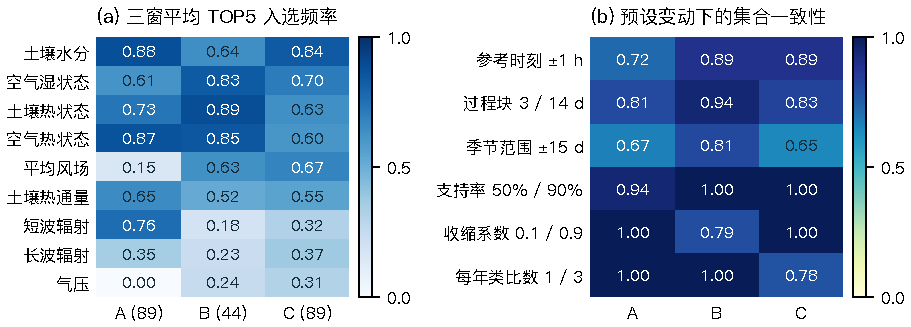
\includegraphics[width=\linewidth]{figures/q1/q1_stability.pdf}
\caption{三路线的重采样稳定性与预设敏感性。左图括号为每窗有效重采样数，请求数均为100；右图按三窗及行内所列变动取TOP5集合Jaccard系数的均值，取值越大表示与主设置越一致。}
\label{q1-fig-stability}
\end{figure}
\FloatBarrier

敏感性同时覆盖参考时刻前后1小时、过程块长度、季节范围、有效支持率、收缩系数与类比配额，全部保留三种窗口，不依据结果挑选最佳窗口。探索轨加入降水及通量信息后，前五项集合保持一致，空气湿与土水的次序互换；部分湍流族的B校准缺少有效贡献，分数保留为空，通量信息据其实际支持范围解释。

短波辐射在A中并列第二，在B和C中的名次下降，提示其异常对比较条件敏感；平均风则由A的第八升至C的第二，体现条件对照的价值。第五席的分歧因此应作为后续机制比较的切入点，分别考察动力交换与地表传热路径，而非按单一路线删去其一。

本问据此向后续分析提供“空气温湿—土壤水热—风与土热通量”的候选结构、变化方向和尺度依赖。区域站观测提供背景约束；源区地形、物源、冰岩结构及孔隙水压力需由空间资料与机理模型共同描述。候选前五项用于安排水热路径的比较，同时保留降水等机制相关输入，由结构稳定性分析判断其在给定源区条件下的作用。
\FloatBarrier
\AIcredit
